\documentclass[11pt,final,hidelinks]{article}
\usepackage[utf8]{inputenc}
\usepackage[T1]{fontenc}
\usepackage{lmodern}
\usepackage[margin=1in]{geometry}
\usepackage[english]{babel}
\usepackage{graphicx}
\usepackage[activate={true,nocompatibility},final,tracking=true,kerning=true,spacing=true,factor=1100,stretch=10,shrink=10]{microtype}
\usepackage{mathtools}
\usepackage{amsmath}
\usepackage{amsthm}
\usepackage{amssymb}
\usepackage{algorithm2e}
% \usepackage{minted} % Disabled - using verbatim instead
\usepackage{booktabs}
\usepackage{hyperref}
\usepackage[square,numbers]{natbib}
\bibliographystyle{plainnat}
\usepackage{cleveref}

% Include unified notation definitions shared across the Bernoulli series
% Unified Notation for Bernoulli Types Research
% =============================================
%
% This file provides consistent notation across all papers based on the
% latent/observed framework that is central to Bernoulli types.
%
% Core Principle: Distinguish between latent (true) and observed (noisy) values

% ========== GENERAL NOTATION ==========

% Latent values (no special decoration - these are the "true" values)
% - x, y, z for elements
% - S, T, U for sets  
% - f, g, h for functions

% Observed values (use tilde to indicate observation/approximation)
% - \obs{x}, \obs{y}, \obs{z} for observed elements
% - \obs{S}, \obs{T}, \obs{U} for observed sets
% - \obs{f}, \obs{g}, \obs{h} for observed functions

\newcommand{\obs}[1]{\widetilde{#1}}  % Universal observation operator

% Alternative: Use \latent and \observed for clarity in definitions
\newcommand{\latent}[1]{#1}
\newcommand{\observed}[1]{\widetilde{#1}}

% ========== BERNOULLI TYPES ==========

% Bernoulli type constructor: B_T^{(k)} following the refined framework
\newcommand{\BType}[1]{B_{#1}}  % Basic Bernoulli type B_T
\newcommand{\BTypeOrder}[2]{B_{#1}^{(#2)}}  % Bernoulli type with order B_T^{(k)}

% Specific Bernoulli types
\newcommand{\BBool}{B_{\mathrm{bool}}}  % Bernoulli Boolean
\newcommand{\BBoolOrder}[1]{B_{\mathrm{bool}}^{(#1)}}  % Bernoulli Boolean with order
\newcommand{\BSet}[1]{B_{#1 \mapsto \mathrm{bool}}}  % Bernoulli set (set indicator function)
\newcommand{\BMap}[2]{B_{#1 \mapsto #2}}  % Bernoulli map from type 1 to type 2

% Latent value notation - B_T(x) represents observation of latent x
\newcommand{\BValue}[2]{B_{#1}(#2)}  % B_T(x) - Bernoulli observation of latent x
\newcommand{\BValueOrder}[3]{B_{#1}^{(#2)}(#3)}  % B_T^{(k)}(x) - with explicit order

% ========== ERROR RATES ==========

% General error terminology (for any type)
\newcommand{\errorrate}{\epsilon}  % Generic error rate
\newcommand{\missrate}{\delta}     % Miss rate (fail to detect when present)
\newcommand{\spuriousrate}{\alpha} % Spurious rate (detect when absent)
\newcommand{\confusionrate}{\gamma} % Confusion between different values

% Boolean-specific terminology (only use for Boolean/binary contexts)
\newcommand{\fprate}{\alpha}  % False positive rate (Boolean only!)
\newcommand{\fnrate}{\beta}   % False negative rate (Boolean only!)
\newcommand{\tprate}{\tau}    % True positive rate (Boolean only!)
\newcommand{\tnrate}{\rho}    % True negative rate (Boolean only!)
\newcommand{\FPR}{\mathsf{FPR}}  % False positive rate (text form)
\newcommand{\FNR}{\mathsf{FNR}}  % False negative rate (text form)

% General approximation error for type T
\newcommand{\ApproxError}[2]{\epsilon_{#1 \to #2}}  % Error from type T1 to T2
\newcommand{\TypeConfusion}[3]{\gamma_{#1}(#2 \to #3)}  % Confusion in type T: value1 -> value2

% Error rate notation for specific structures
\newcommand{\withError}[3]{#1_{#2,#3}}  % e.g., \withError{S}{\spuriousrate}{\missrate}

% ========== ERROR MODEL ORDERS ==========

% Order-2 error model (uniform error rates)
\newcommand{\OrderTwo}{\text{Order-2}}
\newcommand{\UniformError}[2]{\epsilon_{#1}, \delta_{#2}}  % Uniform rates

% Order-|U| error model (element-specific error rates)
\newcommand{\OrderU}{\text{Order-}|\Universe|}
\newcommand{\ElementError}[1]{\text{error}(#1)}  % Element-specific error function
\newcommand{\ElementSpuriousRate}[1]{\spuriousrate_{#1}}   % Element-specific spurious rate
\newcommand{\ElementMissRate}[1]{\missrate_{#1}}           % Element-specific miss rate
% Boolean-specific (only use when appropriate)
\newcommand{\ElementFPRate}[1]{\fprate_{#1}}   % Element-specific false positive (Boolean only!)
\newcommand{\ElementFNRate}[1]{\fnrate_{#1}}   % Element-specific false negative (Boolean only!)

% ========== PROBABILITY AND EXPECTATION ==========

\newcommand{\Prob}[1]{\mathbb{P}\left[#1\right]}
\newcommand{\ProbCond}[2]{\mathbb{P}\left[#1 \mid #2\right]}  % Conditional probability
\newcommand{\Expect}[1]{\mathbb{E}\left[#1\right]}
\newcommand{\Var}[1]{\mathrm{Var}\left[#1\right]}

% ========== INFORMATION THEORY ==========

\newcommand{\Entropy}[1]{H(#1)}  % General entropy H(X)
\newcommand{\ConditionalEntropy}[2]{H(#1 \mid #2)}  % Conditional entropy H(X|Y)
\newcommand{\MatrixEntropy}[1]{H(#1)}  % Matrix entropy H(Q)
\newcommand{\MutualInfo}[2]{I(#1; #2)}  % Mutual information I(X;Y)
\newcommand{\KLDiv}[2]{D_{\mathrm{KL}}(#1 \parallel #2)}  % KL divergence

% ========== SET NOTATION ==========

% Basic sets
\newcommand{\Universe}{\mathcal{U}}  % Universal set
\newcommand{\PowerSet}[1]{\mathcal{P}(#1)}  % Power set
\newcommand{\EmptySet}{\emptyset}

% Set operations (no special commands needed, use standard LaTeX)
% \cup for union
% \cap for intersection  
% \setminus for difference
% \triangle for symmetric difference

% Set operations
\newcommand{\SetUnion}{\cup}
\newcommand{\SetIntersection}{\cap}
\newcommand{\SetComplement}[1]{\overline{#1}}
\newcommand{\Complement}[1]{\overline{#1}}
\newcommand{\PS}[1]{\mathcal{P}(#1)}  % Alternate power set notation

% Cardinality
\newcommand{\Card}[1]{\lvert#1\rvert}

% Membership indicator
\newcommand{\Indicator}[1]{\mathbf{1}_{#1}}

% ========== TYPE NOTATION ==========

\newcommand{\Type}[1]{\mathtt{#1}}

% ========== BOOLEAN VALUES ==========

\newcommand{\Bool}{\mathbb{B}}
\newcommand{\True}{\mathtt{true}}
\newcommand{\False}{\mathtt{false}}

% ========== CHANNEL/CONFUSION MATRIX ==========

% Channel notation: observed | latent
\newcommand{\Channel}[2]{\Prob{\text{observe } #1 \mid \text{latent } #2}}

% Confusion matrix entry
\newcommand{\Confusion}[2]{q_{#1,#2}}  % q_ij = P(observe j | latent i)

% ========== FUNCTION NOTATION ==========

% Function composition (use standard \circ)
% Approximate/observed function application
\newcommand{\ApproxApply}[2]{\obs{#1}(#2)}  % \ApproxApply{f}{x}

% ========== USAGE EXAMPLES ==========

% Example 1: Bernoulli Boolean
% Latent: x \in \Bool
% Observed: \obs{x} \in \Bernoulli{\Bool}{2}
% Relationship: \Channel{\obs{x} = \True}{x = \False} = \fprate

% Example 2: Bernoulli Set  
% Latent: S \subseteq U
% Observed: \obs{S} observes S with rates (\fprate, \fnrate)
% Query: \Channel{x \in \obs{S}}{x \notin S} = \fprate

% Example 3: Composition
% Latent: f \circ g
% Observed: \obs{f} \circ \obs{g}
% Error: \errorrate_{\obs{f} \circ \obs{g}} = \errorrate_f + \errorrate_g - \errorrate_f \errorrate_g

% ========== DEPRECATED NOTATION ==========
% The following should be replaced:
% \ASet{S} → \obs{S}
% \PASet{S} → \obs{S}^+ or \withError{S}{\fprate}{0}  
% \NASet{S} → \obs{S}^- or \withError{S}{0}{\fnrate}
% \Set{S} → S (no decoration needed for latent)

% ========== NOTATION TABLE (for inclusion) ==========

\newcommand{\BernoulliNotationTable}{%
\begin{tabular}{@{}ll@{}}
\textbf{Symbol} & \textbf{Meaning} \\
\midrule
$\obs{x}$ & Observed value corresponding to latent $x$ \\
$\obs{S}$ & Observed (approximate) set for latent $S$ \\
$\obs{f}$ & Observed map approximating latent $f$ \\
$\spuriousrate$ & Spurious rate: $\Prob\{\obs{x}\in\obs{S} \mid x\notin S\}$ \\
$\missrate$ & Miss rate: $\Prob\{\obs{x}\notin\obs{S} \mid x\in S\}$ \\
$\confusionrate$ & Confusion rate between different values \\
$\ElementError{x}$ & Element-specific error function for $x$ \\
$\ElementSpuriousRate{x}$ & Spurious rate specific to element $x$ \\
$\ElementMissRate{x}$ & Miss rate specific to element $x$ \\
$\errorrate$ & Generic error rate $\Prob\{\obs{f}(x)\neq f(x)\}$ \\
$\ApproxError{T_1}{T_2}$ & Approximation error from type $T_1$ to $T_2$ \\
$\TypeConfusion{T}{v_1}{v_2}$ & Confusion in type $T$: value $v_1 \to v_2$ \\
$\fprate, \fnrate$ & False pos./neg. rates (Boolean contexts only) \\
$Q$ & Confusion matrix: $Q_{ij}=\Prob\{\text{obs } t_j\mid \text{lat } t_i\}$ \\
$W(y\mid x)$ & Channel kernel from latent $x$ to observed $y$ \\
$\Entropy{Q}$ & Matrix entropy of confusion matrix $Q$ \\
$\ConditionalEntropy{\text{lat}}{\text{obs}}$ & Conditional entropy of latent given observed \\
$\MutualInfo{X}{Y}$ & Mutual information between $X$ and $Y$ \\
$\Indicator{S}$ & Set indicator function $U\to\Bool$ \\
$\Complement{S}$ & Set complement \\
$\Card{S}$ & Cardinality of a set $S$ \\
\end{tabular}%
}

\newcommand{\NotationSection}{%
\section*{Notation}
This section summarizes symbols used throughout the paper. See also the shared cheat sheet for formulas and assumptions.

\medskip
\noindent\BernoulliNotationTable
}

\usepackage{tikz}
\usetikzlibrary{arrows.meta,positioning}

% Theorem environments
\newtheorem{theorem}{Theorem}[section]
\newtheorem{lemma}[theorem]{Lemma}
\newtheorem{proposition}[theorem]{Proposition}
\newtheorem{corollary}[theorem]{Corollary}
\newtheorem{definition}[theorem]{Definition}
\newtheorem{example}[theorem]{Example}
\newtheorem{remark}[theorem]{Remark}

% Unified notation - defined in unified_notation.tex

% Functions (no decoration for latent, tilde for observed)
\newcommand{\Fun}[1]{\mathsf{#1}}     % Latent function (kept for clarity)
\newcommand{\AFun}[1]{\obs{\mathsf{#1}}}  % Observed function
\newcommand{\PFun}[1]{\mathsf{#1}^*}      % Partial function
\newcommand{\APFun}[1]{\obs{\mathsf{#1}}^*}  % Observed partial function

% Sets (no decoration for latent, tilde for observed)
\newcommand{\Set}[1]{#1}              % Just use S instead of \Set{S}
\newcommand{\ASet}[1]{\obs{#1}}       % Use \obs{S} instead

% Types and probability - defined in unified_notation.tex
% Error rates - defined in unified_notation.tex
\newcommand{\error}{\epsilon}
\newcommand{\Nat}{\mathbb{N}}
\newcommand{\Real}{\mathbb{R}}
\newcommand{\Maybe}[1]{\Type{Maybe}[#1]}
\newcommand{\Unit}{\Type{Unit}}
\newcommand{\Void}{\Type{Void}}
\newcommand{\Nothing}{\mathtt{nothing}}
\newcommand{\Just}[1]{\mathtt{just}(#1)}
% \newcommand{\mapsto}{\rightarrow} % Already defined in LaTeX
\newcommand{\pfun}{\rightharpoonup}
\newcommand{\compose}{\circ}
\newcommand{\Range}{\mathsf{range}}
\newcommand{\Dom}{\mathsf{dom}}
\newcommand{\Cod}{\mathsf{cod}}
\newcommand{\SetIndicator}[1]{\mathbf{1}_{#1}}

\title{Bernoulli Maps: A Universal Framework for Approximate Computation}
\author{
    Alexander Towell\\
    \texttt{atowell@siue.edu}
}
\date{\today}

\begin{document}
\maketitle
\NotationSection

\begin{abstract}
We introduce Bernoulli maps as a general framework for understanding computation through the distinction between latent functions (the true mathematical mappings) and their observations (the computed approximations). Every practical algorithm observes a latent function through a noisy channel—whether due to randomization, resource bounds, or intentional approximation. We show that randomized algorithms, sketching techniques, hash functions, and lossy compression are unified by this perspective: they all implement observed functions that approximate latent mathematical functions with controlled error. By making the latent/observed distinction explicit at the type level, we enable compositional reasoning about error propagation and provide a foundation for designing algorithms with predictable approximation characteristics. The framework reveals that approximation is not a compromise but a fundamental aspect of bridging mathematical functions with computational reality.
\end{abstract}

\section{Introduction}

\subsection{The Latent/Observed Duality in Computation}

In mathematics, functions are perfect mappings from inputs to outputs. In computation, we can only \emph{observe} these latent functions through the lens of finite resources, randomization, and approximation. This fundamental gap between latent mathematical functions and their observed computational implementations appears everywhere:

\begin{itemize}
    \item \textbf{Randomized algorithms} observe latent deterministic functions through random choices
    \item \textbf{Lossy compression} observes latent data through bounded representations
    \item \textbf{Numerical methods} observe latent real functions through floating-point arithmetic
    \item \textbf{Hash functions} observe latent bijections through finite-range mappings
    \item \textbf{Machine learning} observes latent patterns through learned approximations
\end{itemize}

We propose \emph{Bernoulli maps} as a unifying framework that makes this latent/observed distinction explicit. A Bernoulli map is an observed function that approximates a latent function with controlled error probabilities—capturing the reality that computation is fundamentally about observing the unobservable.

\subsection{Motivating Example: Primality Testing}

Consider the problem of testing whether a number is prime. The latent function $\mathsf{isPrime} : \Nat \to \Bool$ is well-defined mathematically but expensive to compute exactly. The Miller-Rabin test \cite{miller1976,rabin1980} provides an \emph{observation} of this latent function in $O(k \log^3 n)$ time.

We model this as observing the latent function through a noisy channel:
\begin{itemize}
    \item \textbf{Latent}: $\mathsf{isPrime}(n)$ - the true primality status
    \item \textbf{Observed}: $\obs{\mathsf{isPrime}}_k(n)$ - Miller-Rabin's output after $k$ rounds
\end{itemize}

The observation quality is characterized by:
\begin{align}
\ProbCond{\obs{\mathsf{isPrime}}_k(n) = \True}{\mathsf{isPrime}(n) = \True} &= 1 \quad \text{(no false negatives)} \\
\ProbCond{\obs{\mathsf{isPrime}}_k(n) = \True}{\mathsf{isPrime}(n) = \False} &\leq 4^{-k} \quad \text{(controlled false positives)}
\end{align}

This exemplifies the key principle: we observe latent mathematical truth through practical computation.

\paragraph{Scope and organization.}  This paper is the third part of our Bernoulli series.  It extends the latent/observed framework from sets (Part~2) to functions by introducing Bernoulli maps.  We build on the foundational definitions of Part~1 (the latent/observed duality and channel models) and the set-theoretic algebra of Part~2 (error propagation through Boolean operations) to develop a universal theory of approximate computation.  Subsequent parts examine regular types (Part~4), information retrieval (Part~5), space–optimal implementations (Part~6), and statistical analysis (Part~7).

\section{Theory of Bernoulli Maps}

\subsection{Basic Definitions}

\begin{definition}[Bernoulli Map]
A Bernoulli map models the observation of a latent function through a probabilistic channel. Given a latent function $f : X \to Y$, an observed function $\obs{f} : X \to Y$ is characterized by the conditional distribution:
\begin{equation}
\ProbCond{\obs{f}(x) = y}{f(x) = y'} = p_{x,y',y}
\end{equation}
This captures how we observe the latent output $f(x) = y'$ as the potentially different value $y$.
\end{definition}

\begin{definition}[Error Profile]
The error profile quantifies the fidelity of observations. For latent $f$ and observed $\obs{f}$, the error at input $x$ is:
\begin{equation}
\error(x) = \Prob{\text{observe } \obs{f}(x) \neq y \mid \text{latent } f(x) = y}
\end{equation}
This measures how often our observation differs from the latent truth.
\end{definition}

\begin{remark}[Interpretation]
Every algorithm that computes a function is effectively providing observations of a latent mathematical function. The error profile characterizes the quality of these observations—whether errors arise from randomization, truncation, or resource bounds.
\end{remark}

\subsection{Confusion Matrix for Functions}

When the domain and codomain are finite, we can represent a Bernoulli map using a confusion matrix, generalizing the concept from classification:

\begin{definition}[Function Confusion Matrix]
For functions of type $X \mapsto Y$ where $|X \mapsto Y| = n$, the confusion matrix $Q \in \mathbb{R}^{n \times n}$ has entries:
\begin{equation}
q_{ij} = \Prob{\text{observe } f_j | \text{latent } f_i}
\end{equation}
where $f_1, \ldots, f_n$ enumerate all functions from $X$ to $Y$.
\end{definition}

\begin{example}[Boolean Function Confusion Matrix]
For $\Bool \mapsto \Bool$, there are 4 functions: $\mathsf{id}$, $\mathsf{not}$, $\mathsf{true}$, $\mathsf{false}$. A first-order Bernoulli approximation has the mini confusion matrix in Figure~\ref{fig:bool-func-confusion}.
\begin{figure}[t]
\centering
\begin{tabular}{c|cccc}
latent \textbackslash observed & $\mathsf{id}$ & $\mathsf{not}$ & $\mathsf{true}$ & $\mathsf{false}$ \\
\hline
$\mathsf{id}$ & $1-\epsilon$ & $\epsilon/3$ & $\epsilon/3$ & $\epsilon/3$ \\
$\mathsf{not}$ & $\epsilon/3$ & $1-\epsilon$ & $\epsilon/3$ & $\epsilon/3$ \\
$\mathsf{true}$ & $\epsilon/3$ & $\epsilon/3$ & $1-\epsilon$ & $\epsilon/3$ \\
$\mathsf{false}$ & $\epsilon/3$ & $\epsilon/3$ & $\epsilon/3$ & $1-\epsilon$
\end{tabular}
\caption{Mini confusion matrix for $\Bool\to\Bool$ under a first-order (symmetric) error model.}
\label{fig:bool-func-confusion}
\end{figure}
This represents a maximum-entropy distribution over off-diagonal errors.
\end{example}

\begin{proposition}[Function Confusion Matrix Properties]
\begin{enumerate}
    \item The order (degrees of freedom) is at most $n(n-1)$ where $n = |Y|^{|X|}$
    \item Function equality probability: $\Prob{\obs{f} = f} = q_{ff}$
    \item Pointwise error accumulates: $\Prob{\obs{f} = f} = \prod_{x \in X} \Prob{\obs{f}(x) = f(x)}$ for independent errors
\end{enumerate}
\end{proposition}

\subsection{Orders of Approximation}

Like Bernoulli sets, Bernoulli maps have different orders based on their error structure:

\begin{definition}[First-Order Bernoulli Map]
A first-order Bernoulli map has uniform error rate:
\begin{equation}
\Prob{\obs{f}(x) \neq f(x)} = \error \quad \forall x \in \Dom(f)
\end{equation}
\end{definition}

\begin{definition}[Second-Order Bernoulli Map]
A second-order Bernoulli map distinguishes between false positives and false negatives:
\begin{align}
\Prob{\obs{f}(x) \neq \bot | f(x) = \bot} &= \fprate \\
\Prob{\obs{f}(x) = \bot | f(x) \neq \bot} &= \fnrate
\end{align}
where $\bot$ represents undefined.
\end{definition}

\subsection{Partial Functions}

Many real-world functions are partial. A partial function $f : X \pfun Y$ can be modeled as a total function $f : X \mapsto \Maybe{Y}$.

\begin{theorem}[Partial Function Approximation]
For a partial function $\PFun{f}$ with domain of definition $\Dom(\PFun{f})$, a Bernoulli approximation $\APFun{f}$ has:
\begin{equation}
\Dom(\APFun{f}) = \ASet{\Dom(\PFun{f})}[\fprate][\fnrate]
\end{equation}
where $\ASet{\cdot}$ denotes a Bernoulli set.
\end{theorem}

\section{Composition of Bernoulli Maps}

\subsection{Sequential Composition}

\begin{theorem}[Error Propagation in Composition]
For Bernoulli maps $\AFun{f} : \Set{X} \mapsto \Set{Y}$ and $\AFun{g} : \Set{Y} \mapsto \Set{Z}$ with error rates $\error_f$ and $\error_g$, the composition $\AFun{g} \compose \AFun{f}$ has error rate bounded by:
\begin{equation}
\error_{g \compose f}(x) \leq \error_f(x) + \error_g(\Fun{f}(x)) - \error_f(x) \cdot \error_g(\Fun{f}(x))
\end{equation}
\end{theorem}

\begin{proof}
The probability of correct computation is:
\begin{align}
\Prob{(\AFun{g} \compose \AFun{f})(x) = (\Fun{g} \compose \Fun{f})(x)} &= \Prob{\AFun{f}(x) = \Fun{f}(x) \land \AFun{g}(\Fun{f}(x)) = \Fun{g}(\Fun{f}(x))} \\
&\geq (1 - \error_f(x))(1 - \error_g(\Fun{f}(x)))
\end{align}
\end{proof}

\subsection{Higher-Order Bernoulli Maps}

Composition naturally produces higher-order approximations:

\begin{definition}[Order of Composition]
The composition of $k$ first-order Bernoulli maps produces a map of order at most $2^k - 1$, as different error paths create distinct distributions.
\end{definition}

\begin{remark}[Non-uniform Error Distribution]
A critical observation: composition destroys the independence assumption of first-order approximations. Elements that pass through different "error paths" in the composition have different error probabilities, making the output errors non-identically distributed. This fundamentally changes the statistical properties and complicates analysis.
\end{remark}

\begin{example}[Iterated Approximation]
Consider iterating a Bernoulli map $\AFun{f}: \Set{X} \to \Set{X}$:
\begin{itemize}
    \item $\AFun{f}^1$: First-order (uniform errors)
    \item $\AFun{f}^2 = \AFun{f} \compose \AFun{f}$: Up to third-order
    \item $\AFun{f}^n$: Exponentially many error classes
\end{itemize}
\end{example}

\subsection{Algebraic Operations on Bernoulli Maps}

For set-indicator functions, we can define algebraic operations:

\begin{theorem}[Set Operation Error Rates]
For Bernoulli approximations of indicator functions $\SetIndicator{A}$ and $\SetIndicator{B}$:
\begin{align}
\text{FPR}(\SetIndicator{A \cap B}) &= \text{FPR}(A) \cdot \text{FPR}(B) \\
\text{FNR}(\SetIndicator{A \cap B}) &= 1 - (1-\text{FNR}(A))(1-\text{FNR}(B)) \\
\text{FPR}(\SetIndicator{A \cup B}) &= 1 - (1-\text{FPR}(A))(1-\text{FPR}(B)) \\
\text{FNR}(\SetIndicator{A \cup B}) &= \text{FNR}(A) \cdot \text{FNR}(B)
\end{align}
under independence assumptions.
\end{theorem}

\begin{proof}
These follow from viewing set operations as Boolean operations on indicator functions and applying error propagation rules for AND/OR operations.
\end{proof}

\subsection{Parallel Composition}

\begin{definition}[Product of Bernoulli Maps]
Given $\AFun{f} : \Set{X} \mapsto \Set{Y}$ and $\AFun{g} : \Set{X} \mapsto \Set{Z}$, the product $\AFun{f} \times \AFun{g} : \Set{X} \mapsto \Set{Y} \times \Set{Z}$ is defined by:
\begin{equation}
(\AFun{f} \times \AFun{g})(x) = (\AFun{f}(x), \AFun{g}(x))
\end{equation}
\end{definition}

\section{Case Studies}

\subsection{Primality Testing as Bernoulli Map}

The Miller-Rabin primality test exemplifies how computational complexity induces the latent/observed distinction:

\begin{example}[Primality as Latent Property]
The function $\mathsf{isPrime}: \mathbb{N} \to \Bool$ is well-defined mathematically but becomes \emph{latent} for large inputs due to computational constraints. The Miller-Rabin test provides an \emph{observation}:
\begin{equation}
\obs{\mathsf{isPrime}}_k \sim \mathcal{B}_{\mathbb{N} \to \Bool}(\mathsf{isPrime})
\end{equation}
where $k$ is the number of witnesses tested.
\end{example}

\begin{algorithm}[H]
\SetAlgoLined
\KwIn{$n > 2$, odd integer; $k$ iterations}
\KwOut{$\True$ if $n$ is probably prime, $\False$ if composite}
Write $n-1 = 2^r \cdot d$ with $d$ odd\;
\For{$i = 1$ to $k$}{
    Choose random $a \in [2, n-2]$\;
    $x \leftarrow a^d \bmod n$\;
    \If{$x = 1$ or $x = n-1$}{continue to next witness}
    \For{$j = 1$ to $r-1$}{
        $x \leftarrow x^2 \bmod n$\;
        \If{$x = n-1$}{continue to next witness}
    }
    \Return $\False$\;
}
\Return $\True$\;
\caption{Miller-Rabin Primality Test}
\end{algorithm}

\begin{theorem}[Miller-Rabin as Bernoulli Map]
The Miller-Rabin test with $k$ iterations yields a second-order Bernoulli map with:
\begin{itemize}
    \item \textbf{False negative rate}: $\beta = 0$ (primes always test as prime)
    \item \textbf{False positive rate}: $\alpha \leq 4^{-k}$ (composites may test as prime)
\end{itemize}
Thus:
\begin{equation}
\Prob{\obs{\mathsf{isPrime}}_k(n) = p | \mathsf{isPrime}(n) = p} = \begin{cases}
1 & \text{if } p = \True \\
\geq 1 - 4^{-k} & \text{if } p = \False
\end{cases}
\end{equation}
\end{theorem}

\begin{remark}[Time-Error Tradeoff]
The Miller-Rabin test trades deterministic exponential time for probabilistic polynomial time with controlled error. Each witness requires $O(\log^3 n)$ time, so $k$ iterations take $O(k \log^3 n)$ time to achieve error rate $4^{-k}$.
\end{remark}

\begin{corollary}[Cryptographic Security]
For 2048-bit RSA key generation, using $k = 40$ witnesses gives:
\begin{equation}
\Prob{\text{composite accepted as prime}} \leq 4^{-40} < 2^{-80}
\end{equation}
meeting standard security requirements.
\end{corollary}

\subsection{Hash Functions}

Hash functions exemplify the latent/observed paradigm: the latent identity function (perfect discrimination of inputs) is observed through a finite-range mapping.

\begin{definition}[Hash Function as Observation]
A hash function $h : X \to [m]$ observes the latent injection $\mathsf{id} : X \hookrightarrow \mathbb{N}$:
\begin{itemize}
    \item \textbf{Latent}: Each $x \in X$ maps to a unique natural number
    \item \textbf{Observed}: $h(x) \in [m]$ provides a finite-precision observation
\end{itemize}
The observation quality for discrimination is:
\begin{equation}
\ProbCond{\obs{(x \neq y)}}{\text{latent } x \neq y} = \Prob{h(x) \neq h(y)} = 1 - \frac{1}{m}
\end{equation}
\end{definition}

\begin{remark}
Hash functions sacrifice perfect injectivity (latent) for finite representation (observed), enabling practical implementations of sets, maps, and caches.
\end{remark}

\subsection{Sketching Algorithms}

Sketching algorithms observe latent frequency distributions through space-bounded data structures:

\begin{definition}[Count-Min Sketch as Observation]
The Count-Min sketch \cite{cormode2005} observes the latent frequency function $\mathsf{freq} : X \to \mathbb{N}$:
\begin{itemize}
    \item \textbf{Latent}: True frequency $\mathsf{freq}(x)$ for each element
    \item \textbf{Observed}: Sketch query $\obs{\mathsf{freq}}_{\epsilon,\delta}(x)$ using $O(\frac{1}{\epsilon} \log \frac{1}{\delta})$ space
\end{itemize}
The observation guarantee:
\begin{equation}
\ProbCond{\obs{\mathsf{freq}}(x) \geq \mathsf{freq}(x)}{\text{any input}} = 1 \quad \text{(no underestimation)}
\end{equation}
\begin{equation}
\ProbCond{\obs{\mathsf{freq}}(x) > \mathsf{freq}(x) + \epsilon \|\mathbf{f}\|_1}{\text{stream } \mathbf{f}} < \delta
\end{equation}
\end{definition}

This shows how we trade space for observation quality: perfect observation would require $O(|X|)$ space, but we achieve useful observations with logarithmic space.

\subsection{Monte Carlo Integration}

Monte Carlo methods approximate integrals through random sampling:

\begin{example}[Monte Carlo Integration]
To approximate $I = \int_a^b f(x) dx$, we use:
\begin{equation}
\AFun{I}_n = \frac{b-a}{n} \sum_{i=1}^n f(X_i)
\end{equation}
where $X_i$ are uniform random samples. This is a Bernoulli map with:
\begin{equation}
\Expect{|\AFun{I}_n - I|^2} = \frac{(b-a)^2 \text{Var}(f)}{n}
\end{equation}
\end{example}

\subsection{Function Equality Testing}

Testing equality of functions demonstrates how sampling creates Bernoulli observations:

\begin{definition}[Approximate Function Equality]
Given functions $f, g: X \to Y$, define the approximate equality test:
\begin{equation}
\obs{(f = g)}_n := \prod_{i=1}^n \mathbf{1}_{f(x_i) = g(x_i)}
\end{equation}
where $x_1, \ldots, x_n \sim \text{Uniform}(X)$.
\end{definition}

\begin{theorem}[Function Equality Error Bounds]
If $f \neq g$ with disagreement set $D = \{x \in X : f(x) \neq g(x)\}$ of size $|D| = k$:
\begin{equation}
\Prob{\obs{(f = g)}_n = \True | f \neq g} = \left(1 - \frac{k}{|X|}\right)^n
\end{equation}
Thus the false positive rate lies in:
\begin{equation}
\alpha \in \left[\left(1 - \frac{|X|-1}{|X|}\right)^n, \left(1 - \frac{1}{|X|}\right)^n\right]
\end{equation}
\end{theorem}

\begin{proof}
The test passes iff all $n$ samples avoid $D$. Since $|D| \geq 1$ when $f \neq g$ and $|D| \leq |X|-1$ (functions must agree on at least one point), we get the bounds.
\end{proof}

\begin{example}[Testing Compiler Optimizations]
To verify that an optimized function $g$ equals the original $f$:
\begin{itemize}
    \item Sample $n = 10^6$ random inputs
    \item If all outputs match: accept with confidence $1 - \alpha$
    \item If any differ: $g \neq f$ with certainty
\end{itemize}
For 32-bit functions, worst-case $\alpha \approx e^{-10^6/2^{32}} \approx 0.9998$, but typical disagreements are more frequent, giving much better confidence.
\end{example}

\section{Computational Trade-offs}

\subsection{Time-Accuracy Trade-off}

Many algorithms exhibit a fundamental trade-off between computation time and accuracy:

\begin{theorem}[Time-Accuracy Trade-off]
For a class of problems with inherent complexity $C$, any algorithm running in time $T < C$ must be a Bernoulli map with error rate:
\begin{equation}
\error \geq 1 - \frac{T}{C}
\end{equation}
\end{theorem}

\subsection{Space-Accuracy Trade-off}

Similarly, space-bounded computation induces approximation:

\begin{theorem}[Space-Accuracy Trade-off]
Any algorithm using space $S$ to represent a set of size $N > 2^S$ must have error rate:
\begin{equation}
\error \geq 1 - \frac{2^S}{N}
\end{equation}
\end{theorem}

\subsection{Communication-Accuracy Trade-off}

In distributed systems, limited communication induces approximation:

\begin{example}[Distributed Mean Estimation]
To compute the mean of $n$ values distributed across $k$ nodes with $B$ bits of communication per node:
\begin{equation}
\error \geq \frac{\sigma^2}{n} \cdot \frac{k}{2^{2B/k}}
\end{equation}
where $\sigma^2$ is the variance.
\end{example}

\section{Codec Theory for Bernoulli Maps}

\subsection{Universal Construction}

We can systematically construct Bernoulli maps through coding theory:

\begin{theorem}[Universal Bernoulli Map Construction]
Given any function $\Fun{f} : \Set{X} \mapsto \Set{Y}$ and error profile $\error$, there exists a Bernoulli map $\AFun{f}$ achieving this profile using:
\begin{equation}
H(\error) + \log |\Set{Y}| \text{ bits per input}
\end{equation}
where $H$ is the binary entropy function.
\end{theorem}

\subsection{Optimal Encoding}

\begin{definition}[Rate-Distortion Function]
For a function $\Fun{f}$ and distortion measure $d$, the rate-distortion function is:
\begin{equation}
R(D) = \min_{p(\hat{y}|x)} I(X; \hat{Y})
\end{equation}
subject to $\Expect{d(\Fun{f}(X), \hat{Y})} \leq D$.
\end{definition}

\subsection{Singular Hash Map: Theoretical Optimality}

We present a theoretical construction achieving information-theoretic bounds:

\begin{definition}[Singular Hash Map]
Given a partial function $\Fun{f}: \Set{X} \pfun \Set{Y}$ and random oracle $h: \Set{X} \times \mathbb{N} \to \{0,1\}^\infty$, the singular hash map:
\begin{enumerate}
    \item Finds seed $s$ such that $\forall x \in \text{dom}(f): h(x,s)|_n = \text{encode}(f(x))$
    \item Stores only the seed $s$
    \item Evaluates $\AFun{f}(x) = \text{decode}(h(x,s)|_n)$
\end{enumerate}
where $|_n$ denotes taking the first $n$ bits.
\end{definition}

\begin{theorem}[Singular Hash Map Properties]
For false positive rate $\fprate = 2^{-k}$ and $m = |\text{dom}(f)|$:
\begin{itemize}
    \item Space: $m(k + \log |Y|)$ bits (information-theoretic optimal)
    \item Construction time: $O(2^{m(k + \log |Y|)})$ expected
    \item Query time: $O(1)$
    \item False negative rate: 0
\end{itemize}
\end{theorem}

\begin{proof}
The probability that a random seed satisfies all constraints is:
\begin{equation}
p = 2^{-m(k + \log |Y|)}
\end{equation}
Thus expected trials until success is $1/p$. The seed itself requires $\log(1/p) = m(k + \log |Y|)$ bits, achieving the entropy bound $H(\fprate) + \log |Y|$ per element.
\end{proof}

\begin{remark}[Practical Considerations]
While theoretically optimal, the exponential construction time makes this impractical. However, it:
\begin{itemize}
    \item Proves achievability of the bound
    \item Suggests relaxations (e.g., allow small false negative rate)
    \item Motivates approximate algorithms targeting this bound
\end{itemize}
\end{remark}

\section{Oblivious Computation}

Bernoulli maps enable privacy-preserving computation:

\begin{definition}[Oblivious Bernoulli Map]
A Bernoulli map $\AFun{f}$ is $\epsilon$-oblivious if for all $x, x' \in \Set{X}$:
\begin{equation}
\frac{\Prob{\AFun{f}(x) = y}}{\Prob{\AFun{f}(x') = y}} \leq e^\epsilon
\end{equation}
\end{definition}

\begin{theorem}[Composition of Oblivious Maps]
The composition of $\epsilon_1$-oblivious and $\epsilon_2$-oblivious Bernoulli maps is $(\epsilon_1 + \epsilon_2)$-oblivious.
\end{theorem}

\subsection{Function Equality Testing}

A fundamental problem is determining whether two functions are equal. The latent truth "$f = g$" is often unobservable directly—we can only observe their behavior on a finite sample of inputs.

\begin{definition}[Observing Function Equality]
Given latent functions $f, g : X \to Y$, we observe their equality through sampling:
\begin{equation}
\obs{(f = g)}_n := \bigwedge_{i=1}^n (f(x_i) = g(x_i))
\end{equation}
where $x_1, \ldots, x_n$ are sampled uniformly from $X$. This provides an observation of the latent equality through $n$ point evaluations.
\end{definition}

\begin{remark}
This exemplifies the latent/observed principle: the latent mathematical fact "$f = g$" can only be observed through finite computation, introducing the possibility of false conclusions.
\end{remark}

\begin{theorem}[Function Equality Error Bounds]
If $f \neq g$ with $k$ points of disagreement in $\Set{X}$, then:
\begin{equation}
\Prob{f \hat{=} g \text{ returns true}} = \left(1 - \frac{k}{|\Set{X}|}\right)^n
\end{equation}
Thus the false positive rate is bounded:
\begin{equation}
\epsilon \in \left[\left(1 - \frac{1}{|\Set{X}|}\right)^n, \left(\frac{n}{|\Set{X}|}\right)^n\right]
\end{equation}
\end{theorem}

\begin{example}[Testing Hash Function Quality]
To verify that a hash function $h : \{0,1\}^{64} \mapsto \{0,1\}^{32}$ behaves randomly:
\begin{verbatim}
bool appears_random(hash_function h, int samples = 10000) {
    // Test uniform distribution
    map<uint32_t, int> counts;
    for (int i = 0; i < samples; i++) {
        uint64_t x = random_uint64();
        counts[h(x)]++;
    }
    
    // Chi-squared test for uniformity
    double chi_squared = compute_chi_squared(counts, samples);
    return chi_squared < critical_value(0.05);
}
\end{verbatim}

This is a Bernoulli approximation of the ideal test that would check all $2^{64}$ inputs.
\end{example}

\section{Implementation Framework}

\subsection{Generic Programming}

We can implement Bernoulli maps generically in C++:

\begin{verbatim}
template <typename X, typename Y>
class bernoulli_map {
public:
    using input_type = X;
    using output_type = Y;
    using error_profile = std::function<double(const X&)>;
    
    virtual Y operator()(const X& x) const = 0;
    virtual double error_rate(const X& x) const = 0;
};

template <typename X, typename Y, typename Z>
class composed_bernoulli_map : public bernoulli_map<X, Z> {
    bernoulli_map<X, Y> f;
    bernoulli_map<Y, Z> g;
public:
    Z operator()(const X& x) const override {
        return g(f(x));
    }
    double error_rate(const X& x) const override {
        // Error propagation formula
        double e_f = f.error_rate(x);
        double e_g = g.error_rate(f(x));
        return e_f + e_g - e_f * e_g;
    }
};
\end{verbatim}

\subsection{Performance Optimizations}

Key optimizations for Bernoulli maps include:
\begin{itemize}
    \item \textbf{Memoization}: Cache results for deterministic approximations
    \item \textbf{Adaptive precision}: Adjust error rates based on context
    \item \textbf{Vectorization}: Process multiple inputs simultaneously
    \item \textbf{GPU acceleration}: Parallelize Monte Carlo sampling
\end{itemize}

\section{Applications}

\subsection{Database Query Optimization}

Approximate query processing uses Bernoulli maps to trade accuracy for speed:

\begin{example}[Approximate COUNT DISTINCT]
Instead of exact counting, use HyperLogLog:
\begin{equation}
\AFun{count}_m(S) = \frac{\alpha_m m^2}{\sum_{j=1}^m 2^{-M[j]}}
\end{equation}
with relative error $\approx 1.04/\sqrt{m}$.
\end{example}

\subsection{Network Function Virtualization}

Network functions can be approximated for performance:

\begin{example}[Approximate Packet Classification]
Replace exact matching with probabilistic filters:
\begin{equation}
\Prob{\AFun{classify}(p) = \Fun{classify}(p)} \geq 1 - \delta
\end{equation}
achieving $O(1)$ classification time.
\end{example}

\subsection{Machine Learning}

Neural networks are Bernoulli maps with learned error profiles:

\begin{example}[Neural Network as Bernoulli Map]
A neural network $\AFun{NN}_\theta : \Real^n \mapsto [k]$ approximates the true labeling function with:
\begin{equation}
\error(x) = \Prob{\AFun{NN}_\theta(x) \neq \Fun{label}(x)}
\end{equation}
minimized during training.
\end{example}

\section{Extension to Relations}

\subsection{Approximate Relations}

While functions are special cases of relations, the framework extends naturally to arbitrary relations:

\begin{definition}[Observed k-ary Relation]
Given a latent k-ary relation $R \subseteq X_1 \times \cdots \times X_k$, an observed relation $\obs{R}$ is a k-ary predicate:
\begin{equation}
\obs{R}: X_1 \times \cdots \times X_k \to \{0,1\}
\end{equation}
with error rates $\alpha$ (false positive) and $\beta$ (false negative) for tuple membership.
\end{definition}

\begin{example}[Approximate Ordering]
For a partial order $\leq$ on set $X$, the observed relation $\obs{\leq}$ satisfies:
\begin{itemize}
    \item If $x \leq y$: $\Prob[\obs{\leq}(x,y) = 1] = 1 - \beta$
    \item If $x \not\leq y$: $\Prob[\obs{\leq}(x,y) = 1] = \alpha$
\end{itemize}
This may violate transitivity: $\obs{\leq}(x,y) \land \obs{\leq}(y,z)$ need not imply $\obs{\leq}(x,z)$.
\end{example}

\begin{proposition}[Non-uniform Error Distribution]
When composing observed relations, errors become non-uniformly distributed. For relations $\obs{R} \subseteq X \times Y$ and $\obs{S} \subseteq Y \times Z$:
\begin{equation}
\obs{S} \circ \obs{R} = \{(x,z) : \exists y \in Y, \obs{R}(x,y) \land \obs{S}(y,z)\}
\end{equation}
The error rate for $(x,z)$ depends on the number of intermediate elements $y$ satisfying the relation.
\end{proposition}

\section{Composition and Error Propagation}

Let $f:X\to Y$ and $g:Y\to Z$ be latent, and let $\obs{f},\obs{g}$ be observed through independent memoryless channels with pointwise error rates $\error_f(x)=\Prob\{\obs{f}(x)\neq f(x)\}$ and $\error_g(y)=\Prob\{\obs{g}(y)\neq g(y)\}$. Consider the composition $h=g\circ f$ with observation $\obs{h}=\obs{g}\circ\obs{f}$.

\begin{proposition}[Union bound for composition]
For any $x\in X$,
\begin{equation}
\Prob\{\obs{h}(x)\neq h(x)\} \;\le\; \error_f(x) + \Expect{\error_g\bigl(f(x)\bigr)}.
\end{equation}
If $\error_f$ and $\error_g$ are bounded by constants $\epsilon_f,\epsilon_g$, then
\begin{equation}
\Prob\{\obs{h}(x)\neq h(x)\} \;\le\; 1-(1-\epsilon_f)(1-\epsilon_g).
\end{equation}
\end{proposition}

\begin{remark}
Channel composition corresponds to matrix multiplication of confusion matrices. The diagonal dominance of the product controls overall fidelity; the simple bound above is often tight enough for design.
\end{remark}

\begin{figure}[t]
\centering
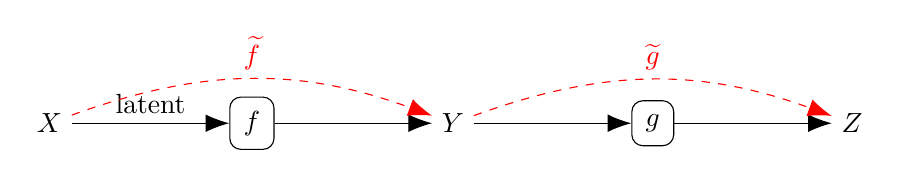
\begin{tikzpicture}[node distance=2.0cm]
  \node (X) {$X$};
  \node (f) [right=of X, draw, rounded corners, inner sep=5pt] {$f$};
  \node (Y) [right=of f] {$Y$};
  \node (g) [right=of Y, draw, rounded corners, inner sep=5pt] {$g$};
  \node (Z) [right=of g] {$Z$};
  \draw[-{Latex[length=3mm]}] (X) -- (f) node[midway, above] {latent};
  \draw[-{Latex[length=3mm]}] (f) -- (Y);
  \draw[-{Latex[length=3mm]}] (Y) -- (g);
  \draw[-{Latex[length=3mm]}] (g) -- (Z);
  \draw[red, dashed, -{Latex[length=3mm]}] (X) to[bend left=20] node[midway, above] {$\obs{f}$} (Y);
  \draw[red, dashed, -{Latex[length=3mm]}] (Y) to[bend left=20] node[midway, above] {$\obs{g}$} (Z);
\end{tikzpicture}
\caption{Function composition with observed channels $\obs{f},\obs{g}$.}
\end{figure}

\subsection{Composition via Confusion Matrices}

For finite codomains, channel composition is algebraic. Let $Y$ be finite and let $W_f(y\mid y')$ be the pointwise channel of $\obs{f}$ and $W_g(z\mid z')$ the pointwise channel of $\obs{g}$. The composed pointwise channel is
\begin{equation}
    W_{g\circ f}(z\mid y') \,=\, \sum_{y\in Y} W_g(z\mid y)\,W_f(y\mid y').
\end{equation}
In particular, if both are binary symmetric channels (BSC) with crossover $\epsilon_f$ and $\epsilon_g$, then $W_{g\circ f}$ is BSC with crossover
\begin{equation}
    \epsilon_{g\circ f} = 1-(1-\epsilon_f)(1-\epsilon_g) = \epsilon_f+\epsilon_g-\epsilon_f\epsilon_g.
\end{equation}

\subsection{Worked Example: $\Bool\to\Bool$}

Let $f(x)=x$ (identity) and suppose we observe $\obs{f}$ through a BSC with $\epsilon_f=0.1$. Let $g(x)=\mathsf{not}(x)$ with observation $\epsilon_g=0.2$. Then for any input $x\in\Bool$,
\begin{equation}
    \Prob\{\obs{(g\circ f)}(x)\neq (g\circ f)(x)\} \le 1-(1-0.1)(1-0.2)=0.28.
\end{equation}
Equivalently, the composed pointwise channel is a BSC with crossover $0.28$.

\paragraph{Sampling equality in the example.} If two Boolean functions disagree on a $\delta=0.1$ fraction of inputs and we sample $n=50$ points uniformly at random, the probability of falsely accepting equality is $\le e^{-0.1\cdot 50} \approx 0.0067$.

\subsection{Related Results}
See Cover and Thomas for channel composition and data-processing inequalities \cite{cover2006}, Motwani and Raghavan for randomized algorithm tail bounds \cite{motwani1995}, and Goldreich for property testing perspectives on function equality \cite{goldreich2017}.

\section{Sampling-Based Function Equality}

Given black-box access to functions $f,g:X\to Y$ over finite $X$, define the disagreement set $D=\{x\in X: f(x)\neq g(x)\}$. The classic sampling test draws i.i.d. $x_1,\dots,x_n\sim\mathrm{Unif}(X)$ and accepts if $f(x_i)=g(x_i)$ for all $i$.

\begin{theorem}[Soundness of sampling equality]
If $|D|/|X|=\delta>0$, then the probability of (falsely) accepting equality is
\begin{equation}
\Prob\{ \forall i,\; f(x_i)=g(x_i) \} \;=\; (1-\delta)^n \;\le\; e^{-\delta n}.
\end{equation}
\end{theorem}

\begin{remark}
In the Bernoulli map setting, the test operates on observations $\obs{f},\obs{g}$; the analysis then compounds with the channels' error rates, yielding slightly looser but still exponential bounds.
\end{remark}

\section{Related Work}

\begin{itemize}
    \item \textbf{Randomized Algorithms}: Motwani and Raghavan \cite{motwani1995} provide comprehensive coverage of randomized algorithms
    \item \textbf{Property Testing}: Goldreich \cite{goldreich2017} studies algorithms that approximate decision problems
    \item \textbf{PAC Learning}: Valiant's framework \cite{valiant1984} for learning approximate concepts
    \item \textbf{Differential Privacy}: McSherry and Talwar \cite{mcsherry2007} on privacy through approximation
\end{itemize}

\section{Conclusions}

Bernoulli maps formalize the fundamental distinction between latent mathematical functions and their computational observations. This framework reveals that every practical algorithm is observing a latent function through the constraints of finite resources, randomization, or intentional approximation.

Key insights from the latent/observed perspective:
\begin{itemize}
    \item \textbf{Unification}: Randomized algorithms, sketches, and hash functions all observe latent functions through different channels
    \item \textbf{Compositionality}: Error propagation laws describe how observation quality degrades through function composition
    \item \textbf{Inevitability}: The gap between latent and observed is not a flaw but an inherent aspect of computation
    \item \textbf{Design principles}: We can systematically construct observations with desired error profiles
\end{itemize}

Future directions include:
\begin{itemize}
    \item Quantum computing: How do quantum observations of latent functions differ?
    \item Synthesis: Can we automatically derive optimal observations given resource constraints?
    \item Hardware: Specialized circuits for common observation patterns
    \item Type systems: Making the latent/observed distinction explicit in programming languages
    \item Machine learning: Neural networks as learned observations of latent functions
\end{itemize}

The universality of Bernoulli maps demonstrates that computation is fundamentally about observing the uncomputable through the lens of the computable.

\bibliography{references}

% Shared one-page cheat sheet at end for quick reference
% Shared appendix: Cheat Sheet for Bernoulli Series
\section*{Appendix: Bernoulli Cheat Sheet}

% Symbols
\paragraph{Symbols}
\begin{tabular}{@{}ll@{}}
$\fprate$ & False positive rate $\Prob\{\obs{x}\in\obs{S}\mid x\notin S\}$ \\
$\fnrate$ & False negative rate $\Prob\{\obs{x}\notin\obs{S}\mid x\in S\}$ \\
$\tprate$ & True positive rate $1-\fnrate$; $\tnrate$: true negative rate $1-\fprate$ \\
$\epsilon$ & Pointwise error for maps: $\epsilon(x)=\Prob\{\obs{f}(x)\neq f(x)\}$ \\
$Q$ & Confusion matrix: $Q_{ij}=\Prob\{\text{obs } t_j\mid \text{lat } t_i\}$ \\
$W(y\mid x)$ & Channel kernel for pointwise observation \\
\end{tabular}

% Set formulas
\paragraph{Bernoulli sets (independent sub-queries)}
\begin{align*}
\fprate_{A\cap B} &= \fprate_A\,\fprate_B, & \fnrate_{A\cap B} &= 1-(1-\fnrate_A)(1-\fnrate_B), \\
\fprate_{A\cup B} &= 1-(1-\fprate_A)(1-\fprate_B), & \fnrate_{A\cup B} &= \fnrate_A\,\fnrate_B, \\
\fprate_{\overline{A}} &= \fnrate_A, & \fnrate_{\overline{A}} &= \fprate_A.
\end{align*}

% Maps formulas
\paragraph{Bernoulli maps}
Composition bound: $\Prob\{\obs{(g\circ f)}\neq g\circ f\} \le 1-(1-\epsilon_f)(1-\epsilon_g)$.  
Channel composition: $W_{g\circ f}(z\mid y')=\sum_y W_g(z\mid y)W_f(y\mid y')$.  
BSC composition: $\epsilon_{g\circ f}=\epsilon_f+\epsilon_g-\epsilon_f\epsilon_g$.

% Bayes / MV
\paragraph{Bayes and aggregation}
Posterior membership: $\displaystyle \Prob\{x\in S\mid x\in \obs{S}\} = \frac{\pi(1-\fnrate)}{\pi(1-\fnrate)+(1-\pi)\fprate}$.  
Majority vote (i.i.d., $\epsilon<\tfrac12$): $\Prob\{\hat{x}_k\neq x\} \le e^{-2(\tfrac12-\epsilon)^2 k}$.

% Intervals
\paragraph{Intervals}
If $\fprate\in[\underline{\alpha},\overline{\alpha}]$ and $\fnrate\in[\underline{\beta},\overline{\beta}]$, propagate by endpoint evaluation due to monotonicity.

% Assumptions
\paragraph{Assumptions}
Unless stated otherwise: (i) memoryless channels (independent across items), (ii) finite alphabets for confusion-matrix arguments, (iii) independence between sub-queries when using product-form laws, (iv) priors specified when applying Bayes.



\end{document}
